\documentclass[11pt,letterpaper]{article}
\topmargin -.5truein
\textheight 9.0truein
\oddsidemargin 0truein
\evensidemargin 0truein
\textwidth 6.5truein
\setlength{\parskip}{5pt}
\setlength\parindent{0pt}
\usepackage[ruled,vlined]{algorithm2e}
\usepackage[table]{xcolor}% http://ctan.org/pkg/xcolor
\usepackage{caption}
\usepackage{subcaption}
\usepackage[round]{natbib}
\usepackage{graphicx}
\usepackage{amsmath}
\usepackage{amssymb}
\usepackage{wrapfig}
\usepackage{dsfont}
\usepackage{multirow}
\usepackage[all]{xy}
\usepackage{tikz}
\usepackage{tikz-qtree}
\usepackage{drs}

\newcommand{\bs}{\textbackslash}
\renewcommand{\vec}[1]{\mathbf{#1}}
\newcommand{\sem}[1]{\mbox{[\hspace{-1.25px}[{\bf #1}]\hspace{-1.5px}]}}
\newcommand{\sub}[1]{$_{#1}$}

\renewcommand\drsalignment{l}

\usepackage{hyperref}
\hypersetup{
    colorlinks,
    citecolor=black,
    filecolor=black,
    linkcolor=black,
    urlcolor=black
}

\title{NLP: Computational Semantics}
\author{Dan Garrette\\\small{dhg@cs.utexas.edu}}

\begin{document}
\maketitle



\section{First-Order Logic}

\begin{itemize}
  \item $P \land Q$: $P$ and $Q$ are both true
  \item $P \lor Q$: Either $P$ is true or $Q$ is true or both are true
  \item $P \Rightarrow Q$: If $P$ is true, then $Q$ must also be true
  \item $\lnot P$: $P$ is false
  \item $\forall x.P(x)$: For all $x$, $P(x)$ is true
  \item $\exists x.P(x)$: There exists an $x$ such that $P(x)$ is true
\end{itemize}

\section{Lambda Calculus}

\begin{itemize}
  \item $\lambda x.f(x)$: An anonymous function that takes $x$ as an argument and returns $f(x)$
  \item $\beta$-reduction: When the function $\lambda x.f(x)$ is applied some value $y$, we insert $y$ for each occurrence of $x$.  So, $(\lambda x.f(x))(y)$ becomes $f(y)$.
  \item $\alpha$-conversion: Since the $x$ in $\lambda x.f(x)$ is just the name of a parameter, we can replace it with any other parameter name.  So $\lambda x.f(x)$ can be rewritten as $\lambda y.f(y)$.
\end{itemize}


\section{Semantics}

\begin{itemize}
  \item Richard Montague
  \item Principle of Compositionality: the meaning of an expression is the the combination of the meanings of its parts.
\end{itemize}


Proper nouns are ``individuals''.  

~~~~ \sem{Mary}: $\textit{mary}'$

Intransitive verbs are functions over ``individuals'', saying that the individual does that thing.  Individuals are always represented with a lower-case variable.  Functions over individuals are called ``properties''; they indicate that the individual ``has that property''.

~~~~ \sem{sleeps}: $\lambda x.\textit{sleeps}'(x)$

Example: ``Mary sleeps''

\begin{itemize}
  \item[] \sem{Mary sleeps}: \sem{sleeps}(\sem{Mary}) = $(\lambda x.\textit{sleeps}'(x))(\textit{mary}')$ 
                                                      = $\textit{sleeps}'(\textit{mary}')$
\end{itemize}

So \textit{Mary} has the property of \textit{sleeping}.

Transitive verbs are functions over individuals that produce a new function over individuals.  So a transitive verb takes a first individual and produces a new function that looks something like an intransitive verb.

~~~~ \sem{sees}:~ $\lambda x.\lambda y.\textit{sees}'(y,x)$

Example: ``Mary sees Bill''
  \begin{align*}
     \sem{Mary sees Bill}:~ & (\sem{sees}(\sem{Bill}))(\sem{Mary})  \\
                            & ((\lambda x.\lambda y.\textit{sees}'(y,x))(\textit{bill}'))(\sem{Mary}) \\
                            & (\lambda y.\textit{sees}'(y,\textit{bill}'))(\textit{mary}') \\
                            & \textit{sees}'(\textit{mary}',\textit{bill}')
  \end{align*}

We can see that \textit{sees} applies first to the direct object \textit{Bill} to produce a property that looks like an intransitive verb \textit{sees\_Bill}.  This new function applies to the subject \textit{Mary} to indicate that Mary has the property of seeing Bill.


\section{Syntax-driven semantics (with CCG)}

Up until this point, we have seen that each word in a sentence can have an associated meaning representation, and that those meaning can be composed to get the meanings of larger phrases, but we have not given any indication of how we know the order in which these pieces should be composed.  One natural way is to use syntax to drive this process since, after all, the syntax of a sentence determines how we read its meaning.

In CCG, every token has an associated CCG category.  We can extend this to use semantics by attaching the meaning of the token to its category.

\Tree [.{S : \underline{~~~~~~~~~~~~~~~~~~~~~~~~~~~}}
        [.{NP : $\textit{mary}'$} Mary ] 
        [.{S\bs NP : \underline{~~~~~~~~~~~~~~~~~~~~~~~~~~~}} 
          [.{(S\bs NP)/NP : $\lambda x.\lambda y.\textit{sees}'(y,x)$} sees ] 
          [.{NP : $\textit{bill}'$} Bill ] 
        ] 
      ]

Now we can use the category combinations to drive the semantics combinations.  

The tree tells us that \textit{sees} combines first with \textit{Bill}, and that \textit{sees} is the function and \textit{Bill} is the argument (since the category of \textit{sees} is (S\bs NP)/NP, which takes an NP argument to its right, which is exactly what \textit{Bill} is).  So just as the category of \textit{sees} applies to the category of \textit{Bill} to produce a combined category (S \bs NP), the semantics of \textit{sees} applies to the semantics of \textit{Bill} to produce a combined semantics:

\Tree [.{S : \underline{~~~~~~~~~~~~~~~~~~~~~~~~~~~}}
        [.{NP : $\textit{mary}'$} Mary ] 
        [.{S\bs NP : $\lambda y.\textit{sees}'(y,\textit{bill}')$} 
          [.{(S\bs NP)/NP : $\lambda x.\lambda y.\textit{sees}'(y,x)$} sees ] 
          [.{NP : $\textit{bill}'$} Bill ] 
        ] 
      ]

This process continues for the combination of \textit{Mary} and \textit{sees Bill}.

\Tree [.{S : $\textit{sees}'(\textit{mary}',\textit{bill}')$} 
        [.{NP : $\textit{mary}'$} Mary ] 
        [.{S\bs NP : $\lambda y.\textit{sees}'(y,\textit{bill}')$} 
          [.{(S\bs NP)/NP : $\lambda x.\lambda y.\textit{sees}'(y,x)$} sees ] 
          [.{NP : $\textit{bill}'$} Bill ] 
        ] 
      ]


\section{Quantification}

Nouns are functions over individuals that say that that individual has the property of being that noun.

~~~~ \sem{dog}: $\lambda x.\textit{dog}'(x)$

Quantifiers are functions over two properties.  Property variables are written with upper-case letters.

The semantics of a \textbf{universal quantifier} like \textit{every} takes two properties and says that every individual that has the first property must also have the second property:

~~~~ \sem{every}: $\lambda P.\lambda Q.\forall x.[ P(x) \Rightarrow Q(x) ]$

The semantics of an \textbf{existential quantifier} like \textit{a} takes two properties and says that there is some individual that has both the first property and the second property:

~~~~ \sem{a}: $\lambda P.\lambda Q.\exists x.[ P(x) \land Q(x) ]$

Example: ``every dog barks''
  \begin{align*}
     \sem{every dog barks}:~ & (\sem{every}(\sem{dog}))(\sem{barks})  \\
                             & (\lambda P.\lambda Q.\forall x.[ P(x) \Rightarrow Q(x) ])(\lambda z.\textit{dog}'(z))(\sem{barks}) \\
                             & (\lambda Q.\forall x.[ (\lambda z.\textit{dog}'(z))(x) \Rightarrow Q(x) ])(\sem{barks}) \\
                             & (\lambda Q.\forall x.[ \textit{dog}'(x) \Rightarrow Q(x) ])(\sem{barks}) \\
                             & (\lambda Q.\forall x.[ \textit{dog}'(x) \Rightarrow Q(x) ])(\lambda y.\textit{barks}'(y)) \\
                             & \forall x.[ \textit{dog}'(x) \Rightarrow (\lambda y.\textit{barks}'(y))(x) ] \\
                             & \forall x.[ \textit{dog}'(x) \Rightarrow \textit{barks}'(x) ]
  \end{align*}

And with the syntax driving the derivation:

\Tree [.{S : $\forall x.[ \textit{dog}'(x) \Rightarrow \textit{barks}'(x) ]$} 
        [.{NP : $\lambda Q.\forall x.[ \textit{dog}'(x) \Rightarrow Q(x) ]$}
          [.{NP/N : $\lambda P.\lambda Q.\forall x.[ P(x) \Rightarrow Q(x) ]$} every ]
          [.{N : $\lambda x.\textit{dog}'(x)$} dog ]
        ] 
        [.{S\bs NP : $\lambda y.\textit{barks}'(y)$} barks ] ] 


\section{Semantic Ambiguity}

Semantic ambiguity is possible even when the syntax is unambiguous.  For example: ``every student took a test'' has exactly one syntacic parse, but it has two semantic interpretations:

\begin{itemize}
  \item[] \sem{every}(\sem{student}, \sem{a}(\sem{test}, \sem{took})): 
  $\forall s.[\textit{student}'(s) \Rightarrow \exists t.[test(t) \land took(s,t)]]$
  \item[] \sem{a}(\sem{test}, \sem{every}(\sem{student}, \sem{took})): 
  $\exists t.[test(t) \land \forall s.[\textit{student}'(s) \Rightarrow took(s,t)]]$
\end{itemize}

Semantic ambiguities are more complex to handle, but several frameworks exist to manage them.  Generally these use \textbf{underspecified} semantic representations that capture some of the semantic structure while leaving some portions incomplete (though contrained to still be legal representations).

One underspecification framework is \textbf{Hole Semantics} developed by Johan Bos.  The basic idea is that you have ``labels'' on logical expression, ``holes'' in the expression, and constriants on which holes can be filled by which labels:

\begin{itemize}
  \item[] $l_1: \forall s.[student(s) \Rightarrow h_1]$
  \item[] $l_2: \exists t.[test(s) \Rightarrow h_2]$
  \item[] $l_3: \lambda x.\lambda y.took(x,y)$
  \item[] $l_1 \leq h_0$
  \item[] $l_2 \leq h_0$
  \item[] $l_3 \leq h_1$
  \item[] $l_3 \leq h_2$
\end{itemize}


\section{Neo-Davidsonian Semantics}

In our current view of logical forms, we may see representations like this:

\begin{itemize}
  \item[] \sem{Mary helped}: $\textit{help}'(\textit{mary}')$
  \item[] \sem{Mary helped Bill}: $\textit{help}'(\textit{mary}', \textit{bill}')$
  \item[] \sem{Mary helped Bill with homework}: $\textit{help}'(\textit{mary}', \textit{bill}', \textit{homework}')$
  \item[] \sem{Mary helped with homework}: $\textit{help}'(\textit{mary}', \textit{homework}')$
\end{itemize}

But this scheme is problematic because it is inflexible and doesn't capture the generalities among these statements.  In this scheme the logical form of \textit{Mary helped Bill with homework} does not entail the logical form of \textit{Mary helped Bill}.

Neo-Davidsonian semantics tries to fix this problem by separating out all of the verb's arguments.  It does this by shifting the focus to a discussion about \textbf{events} and makes statements about those events.  So now the statement ``Mary helped'' is given a representation that states that there is some event $e$ that is a ``helping'' event and that Mary is doing the helping:

~~~~ \sem{Mary helped}: $\exists e.[\textit{help}'(e) \land \text{agent}(e, \textit{mary}')]$

Therefore, all other arguments to the verb are simply additional conjuncts:

\begin{itemize}
  \item[] \sem{Mary helped Bill}: $\exists e.[\textit{help}'(e) \land \text{agent}(e, \textit{mary}') \land \text{patient}(e, \textit{bill}')]$
  \item[] \sem{Mary helped Bill with homework}: $\exists e.[\textit{help}'(e) \land \text{agent}(e, \textit{mary}') \land \text{patient}(e, \textit{bill}') \land \\ \text{theme}(e, \textit{homework}')]$
  \item[] \sem{Mary helped with homework}: $\exists e.[\textit{help}'(e) \land \text{agent}(e, \textit{mary}') \land \text{theme}(e, \textit{homework}')]$
\end{itemize}

And, according to the rules of first order logic, the representation of \textit{Mary helped Bill with homework} entails the representation of \textit{Mary helped Bill}:

~~~~ $\exists e.[\textit{help}'(e) \land \text{agent}(e, \textit{mary}') \land \text{patient}(e, \textit{bill}') \land \text{theme}(e, \textit{homework}')] \vDash \exists e.[\textit{help}'(e) \land \text{agent}(e, \textit{mary}') \land \text{patient}(e, \textit{bill}')]$


\subsubsection{Neo-Davidsonian Semantics and Dependency Grammar}

Using (labeled) dependency grammars makes generating Neo-Davidsonian representations straightforward:

\begin{figure}[h]
  \centering
  \begin{subfigure}[b]{0.4\textwidth}
  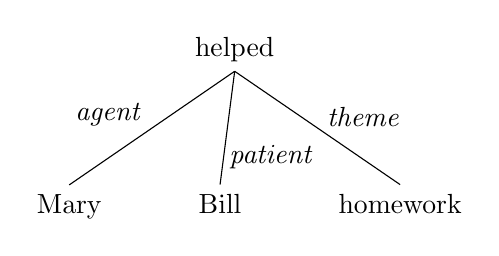
\begin{tikzpicture}
  \tikzset{level distance=20mm, sibling distance=10mm}
    \Tree
      [.helped 
        \edge node[auto=right, yshift=-1mm]{\textit{agent}}; [.{Mary} ]
        \edge node[auto=left,  yshift=-1mm, xshift=-1mm]{\textit{patient}}; [.{Bill} ]
        \edge node[auto=left,  yshift=-1mm]{\textit{theme}}; [.{homework} ]
      ]
  \end{tikzpicture}      
  \caption{Mary helped Bill with homework.}
  \end{subfigure}%
  ~~~~~~~ ~~
  \begin{subfigure}[b]{0.4\textwidth}
  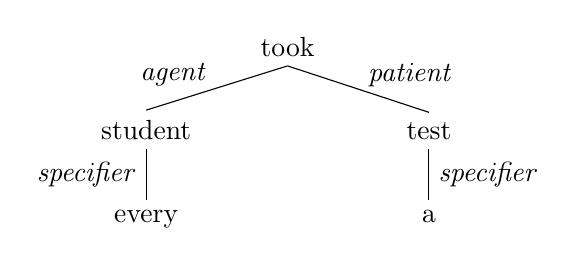
\begin{tikzpicture}
  \tikzset{sibling distance=25mm}
    \Tree
      [.took 
        \edge node[auto=right, yshift=-1mm]{\textit{agent}}; [.{student} 
          \edge node[auto=right]{\textit{specifier}}; [.{every} ] ]
        \edge node[auto=left, yshift=-1mm]{\textit{patient}}; [.{test}
          \edge node[auto=left]{\textit{specifier}}; [.{a} ] ]
      ]
  \end{tikzpicture}      
  \caption{Every student took a test.}
  \end{subfigure}
\end{figure}


\section{Discourse Representation Theory (DRT)}

DRT is a similar to first-order logic, but it differs in a few key ways.  First, expressions in DRT are written in a graphical format known as a Discourse Representation Structure (DRS).  Second, DRT is a \textit{dynamic} logic, meaning that the expressions can be \textit{updated} as more information is available (ie, as more text is read).

A DRS consists of two parts written inside a ``box''.  On top are the \textit{discourse referents}, which are basically existentially quantified variables.  Below are the \textit{discourse conditions}, which are logical statements.

Examples:
\begin{align*}
  \sem{fido barks}  &= \drs{ }{barks(fido)} \\
  \sem{a dog barks} &= \drs{x}{dog(x) \\ barks(x)}
\end{align*}

A pronoun would be represented in DRT as a variable whose antecedent must be resolved:
\begin{align*}
  \sem{he walks} &= \drs{x}{walks(x) \\ x = ?}
\end{align*}


DRT becomes particularly interesting as we add more information (new sentences) to the discourse.  When we add a new sentence, we ``merge'' it into the existing discourse by adding its referents to the existing set of referents and adding its conditions to the existing set of conditions.  Once the new sentence is merged in, any unbound pronouns \textit{in the new sentence} can be resolved.

\begin{align*}
  \sem{A dog barks. He walks.} &= \drs{x}{dog(x) \\ barks(x)} \oplus \drs{y}{walks(y) \\ y = ?}
                                = \drs{x y}{dog(x) \\ barks(x) \\ walks(y) \\ y = x}
\end{align*}

Note, however, that pronouns can only be resolved to ``accessible'' referents, which are referents in the current box or any out-scoping box.  Thus, the pronoun in this discourse fails to resolve:

\begin{align*}
  \sem{No dog barks. He walks.} &= \drs{ }{\negdrs{x}{dog(x) \\ barks(x)}} \oplus \drs{y}{walks(y) \\ y = ?}
                                 = \drs{y}{\negdrs{x}{dog(x) \\ barks(x)} \\ walks(y) \\ y = ?} \\
  \sem{Every dog barks. He walks.} &= \drs{ }{\ifdrs{x}{dog(x)}{ }{barks(x)}} \oplus \drs{y}{walks(y) \\ y = ?}\\
                                   &= \drs{y}{\ifdrs{x}{dog(x)}{ }{barks(x)} \\ walks(y) \\ y = ?}
\end{align*}


\section{Textual Entailment}

Typically, when we are working in semantics, we don't merely want to represent meanings, we usually want to use those meanings to perform tasks.  

One such task is \textit{textual entailment}, which is determining whether one piece of text entails another.  Converting to logical form allows us to use standard first-order theorem proving to determine whether one text entails another:

\begin{align*}
  \text{``Fido barks and sleeps.''} &\vDash \text{``Fido barks.''} \\
  \textit{barks}'(\textit{fido}') \land \textit{sleeps}'(\textit{fido}') &\vDash \textit{barks}'(\textit{fido}')
  \\\\
  \text{``Fido barks.''} &\not\vDash \text{``Fido barks and sleeps.''} \\
  \textit{barks}'(\textit{fido}') &\not\vDash \textit{barks}'(\textit{fido}') \land \textit{sleeps}'(\textit{fido}')
  \\\\
  \text{``Every dog barks.''} &\vDash \text{``A dog barks.''} \\
  \forall x.[\textit{dog}'(x) \Rightarrow \textit{barks}'(x)] &\vDash \exists x.[\textit{dog}'(x) \land \textit{barks}'(x)]
  \\\\
  \text{``A dog barks.''} &\vDash \text{``Every dog barks.''} \\
  \exists x.[\textit{dog}'(x) \land \textit{barks}'(x)] &\vDash \forall x.[\textit{dog}'(x) \Rightarrow \textit{barks}'(x)]
  \\\\
  \text{``Every dog barks.''} &\vDash \text{``Fido is a dog and fido barks.''} \\
  \forall x.[\textit{dog}'(x) \Rightarrow \textit{barks}'(x)] &\vDash 
  \textit{dog}'(\textit{fido}') \land \textit{barks}'(\textit{fido}')]
\end{align*}


\section{Issues with Logical Semantics}

The principle of compositionality doesn't hold for idioms:
\begin{align*}
  \text{``Bill kicked the bucket.''} &\vDash? \text{``A bucket was kicked.''} \\
\end{align*}

It doesn't handle word sense:
\begin{align*}
  \text{``The player picked up the bat.''} &\vDash? \text{``The player picked up an animal.''} \\
  \text{``The bat flew out of the cave.''} &\vDash? \text{``A baseball bat few out of a cave.''} \\
\end{align*}

It doesn't have any notion of likelihood.  
\begin{itemize}
  \item In some contexts it may be ambiguous whether an idiom is being used or not.
  \item In some contexts two sense may be \textit{possible}, one sense may be more likely than another.
\end{itemize}




\end{document}

